


\begin{KR}{Flächeninhalt bei wechselndem Vorzeichen von $f(x)$}\\
\begin{itemize}
  \item $[a, b]=$ Intervall
  \item $x_{1}, x_{2}, \ldots, x_{n}=$ Nullstellen
\end{itemize}

$$\left|\int_{a}^{x_{1}} f(x) d x\right|+\left|\int_{x_{1}}^{x_{2}} f(x) d x\right|+\cdots+\left|\int_{x_{n}}^{b} f(x) d x\right|$$
\end{KR}

\begin{center}
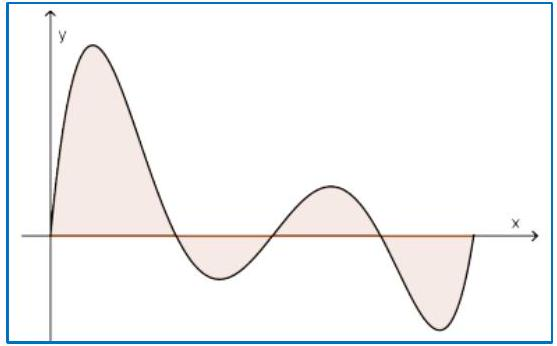
\includegraphics[scale=0.25]{Analysis1/zsf/Images/Integral/2024_01_20_7bfda6c084929ccc01ffg-06(1).jpg}
\end{center}

\begin{KR}{Flächeninhalt zwischen zwei Kurven $f(x)$ und $g(x)$}\\
\begin{itemize}
  \item $[a, b]=$ Intervall
  \item $x_{1}, x_{2}, \ldots, x_{n}=$ Schnittpunkte
\end{itemize}
$$\left|\int_{a}^{x_{1}}(f(x)-g(x)) d x\right|+\left|\int_{x_{1}}^{x_{2}}(f(x)-g(x))\right|+\cdots+\left|\int_{x_{n}}^{b}(f(x)-g(x))\right|$$
\end{KR}

\begin{center}
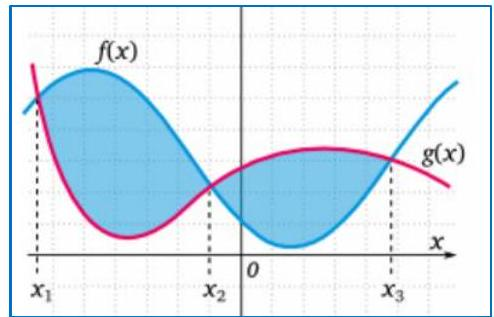
\includegraphics[scale=0.25]{Analysis1/zsf/Images/Integral/2024_01_20_7bfda6c084929ccc01ffg-06(2).jpg}
\end{center}

